
\section{Fachliche Grundlagen}

Dieses Kapitel beschäftigt sich vor allem mit Quelltext. Wer schreibt ihn, wie wird er erstellt, wie sieht er aus, welche Entwicklungen hat es dabei gegeben. Was gibt es für Ansätze um einen langen Quelltext einheitlich aussehen zu lassen und vor allem wodurch zeichnet sich guter Quelltext aus und was sind die Auswirkungen von schlechtem. Zu guter Letzt werfen wir noch einen Blick auf die Wörter \enquote{Art} und \enquote{Science}, die in diesem Zusammenhang oft verwendet werden.

\subsection{Quelltext und der Autor}

Quelltext ist eine für den Computer verständliche Form
eines Arbeitsablaufes. Er kann durch einen Compiler in Maschinencode übersetzt werden.
In den meisten Fällen ist er in Textform verfasst und für den Menschen lesbar.

In einem Softwareprojekt ist er die detaillierteste Spezifikation der zu erstellenden
Software und all ihrer Komponenten. Alles wird in ihm so eindeutig beschrieben,
dass ein Computer ihn umsetzen kann. Das aus der modellgetriebenen Entwicklung
bekannte UML hat das Ziel den Quelltext durch definierte Modelle zu ersetzen.
Diese sind aus heutiger Sicht aber noch nicht als Quelltext Ersatz geeignet,
da die UML nicht genau genug ist und in ihr bestimmte Implementierungsdetails verloren gehen.
 \cite[S. 26]{Martin}

Der Autor dieser genauesten Spezifikation, des Quelltextes, ist der Programmierer.

\subsection{Wandel in der Entwicklung von Quelltexten}


In den Anfängen des Computerzeitalters war der Programmierer meistens der einzige
Leser seiner Programme. Hauptaugenmerk lag auf der Funktion des Programmes
und dem effizienten Umgang mit den Ressourcen, die zu dieser Zeit noch sehr knapp waren.
 Damals gab es noch keine Objekt-Orientierten-Sprachen. Zudem waren die Arbeitsumgebungen der Entwickler
wesentlich bescheidener als in der heutigen Zeit. Quelltexte wurden im ASCII-Code
kodiert und es passten lediglich 80 Zeichen auf eine Bildschirmzeile.

Durch die rasante technische Weiterentwicklungen ist ein Programmierer heutzutage keiner
80 Zeichen Zeile mehr unterworfen. Auch muss nicht mehr auf jedes Bit Speicherverbrauch
optimiert werden. Die Werkzeuge zur Softwareentwicklung haben sich auch verbessert. So
werden heutzutage leistungsfähige IDEs verwendet, deren Funktionsumfang weit über ein
einfaches Syntaxhighlighting hinausgeht. Funktionen wie eine automatische Codevervollständigung
gehören mittlerweile zum Standard. Zudem kommen unzählige, frei verfügbare Bibliotheken und Quelltexte
für eine Vielzahl von Problemen, die über das Internet bezogen werden können. Das Internet bietet zudem
eine solide Quelle für die Recherche nach möglichen Lösungen und Problemlösungsansätzen, sowie
umfangreicher Dokumentation zu Programmiersprachen, Programmierwerkzeugen und eingesetzten Bibliotheken.

\subsection{Programmarten}

Es gibt viele verschiedene Programme, die sich auf unterschiedliche Weise kategorisieren lassen. Im Kontext dieser Arbeit lassen sie sich in drei Kategorien einordnen.

Zur ersten zählen kleine Programme bzw. Skripte, die für den einmaligen
Gebrauch bestimmt sind. Eine einmalige Migration von Daten, in ein bestehendes
oder neues System, fallen in diese Kategorie. Die Programme haben nur einen
geringen (Quelltext-)Umfang und lassen sich von daher schnell überschauen. Sie weisen zudem eine geringe Komplexität auf. Da sie auch nur einmalig angewandt werden ist der Autor zugleich auch der einzige Leser.

Zur zweiten Kategorie gehören Programme aus der Lehre. Es handelt sich hier um Programme die hauptsächlich der Veranschaulichung dienen. Diese haben meist eine
deutlich höhere Dichte an Kommentaren als es für einen Quelltext der anderen
beiden Kategorien der Fall ist. Im Extremfall gibt es hier mehr Kommentarzeilen als eigentliche Zeilen Quelltext.  Sie dienen häufig dazu jede Zeile des Quelltextes direkt zu erklären.

Die dritte Kategorie beherbergt Anwendungen die eine längere Zeit im Einsatz sind.
Sie werden nicht von einem einzelnen Entwickler erstellt sondern von einem ganzen Team. Dazu gehört auch eine gewisse Fluktuation im Team. Die Entwickler führen Weiterentwicklungen durch und warten die Software. Die Arbeit richtet sich vor allem an die dritte Kategorie von Software, da der Quelltext von mehreren Entwicklern gelesen und 
verstanden werden.

\subsection{Formatierung von Quelltexten}


Die Formatierung eines Quelltextes mit korrekter Syntax wird durch
sogenannte Whitespaces (nicht sichtbare Zeichen) vorgenommen.
Dazu gehören Tabulatoren, Leerzeichen und Zeilenumbrüche. Sie dienen dazu den Quelltext für den Menschen lesbarer zu machen.

\begin{listing}[H]
    \begin{minted}{c}
#include <stdio.h>
int main(void){printf("Hello World!");return 0;}
    \end{minted}
    \caption{\enquote{Hello World} Programm in C mit minimalen Whitespaces}
    \label{grundlagen:hellocminimal}
\end{listing}

Für einen Compiler machen Whitespaces häufig keinen Unterschied, Ausnahmen wie die Programmiersprache \enquote{Whitespace} bestätigen die Regel.\footnote{siehe auch http://compsoc.dur.ac.uk/whitespace/}
Es ist egal ob der Quelltext viele Whitespaces enthält, wie in Listing \ref{grundlagen:helloc}), oder nur minimale, wie in Listing \ref{grundlagen:hellocminimal}.
Der Zeilenumbruch in Zeile 1 im Listing \ref{grundlagen:helloc} ist hier Teil der Syntax.

Für den Entwickler tragen die Whitespaces zur Lesbarkeit des Programmes bei. Listing \ref{grundlagen:helloc} ist für einen Menschen besser verständlich, da sich mit den Whitespaces die Struktur abbilden lässt. Der Anfang und das Ende der \texttt{main}-Methode sind so gut zu erkennen.

\begin{listing}[H]
    \begin{minted}{c}
#include <stdio.h>

int main(void) {
    printf("Hello World!");
    return 0;
}
    \end{minted}
    \caption{\enquote{Hello World} Programm in C mit Whitespaces}
    \label{grundlagen:helloc}
\end{listing}

Ein kontrovers diskutiertes Thema ist die Positionierung von öffnenden
und schließenden Blockklammern.
In Listing \ref{grundlagen:blockklammern} sind die drei gängigsten
Arten der Positionierung zu sehen. Obwohl sie alle verschieden sind, verfolgen
sie dennoch dasselbe Ziel, die Struktur durch Einrückungen zu verdeutlichen.

\begin{listing}[H]
        \begin{minipage}{0.35\textwidth}
            \centering
	    \begin{minted}{c}
if (expression) {
    statements
}
	    \end{minted}
        \end{minipage}
        \begin{minipage}{0.3\textwidth}
            \centering
	    \begin{minted}{c}
if (expression)
{
    statements
}
	    \end{minted}
        \end{minipage}
        \begin{minipage}{0.3\textwidth}
            \centering
	    \begin{minted}{c}
if (expression)
	{
    statements
	}
	    \end{minted}
        \end{minipage}
    \caption{Positionierung von Blockklammern aus \cite[S. 8]{Green}}
    \label{grundlagen:blockklammern}
\end{listing}

Aufgrund des Vergleiches, wie sehr Quelltext schreiben mit dem früheren Schreibmaschinenschreiben übereinstimmt, von Kamp\cite{Kamp} kommt man zu der Erkenntnis, dass Quelltext immer in einer Monospace Schriftart geschrieben werden sollte\cite[S. 2]{Green}. Dadurch funktioniert zum einen die Einrückung und zum anderen lassen sich damit Programme in Tabellenform schreiben. Ein Beispiel ist in Listing \ref{grundlagen:tablecode} zu sehen.

\begin{listing}[H]
    \begin{minted}{java}
int color      = 255;
long width     = 400320;
String caption = "Beschreibender text";
    \end{minted}
    \caption{Tabellendarstellung in Quelltext}
    \label{grundlagen:tablecode}
\end{listing}

Das Hinzufügen von Whitespaces um die Lesbarkeit eines Textes zu verbessern, ist in der Typographie nichts Neues. Deren Repertoire reicht weit über Zeilenumbrüche und Leerzeichen hinaus. Unter anderem gibt es in der Typographie den Grauwert. Der Grauwert ist u.a. ausschlaggebend für den Gesamteindruck und die Lesbarkeit
eines Textes. Er beschreibt das Verhältnis zwischen den schwarzen Anteilen, der Schrift, und den Weißen. Im Allgemeinen ist bei einem Quelltext der Grauwert höher als bei einem Buch.  \cite{Beinert}


\subsection{Namensgebung}

Beim Erstellen von Quelltext gibt es viele Vorgaben, bei denen der Autor nicht von den Vorgaben der Programmiersprache abweichen darf, wie die Syntax der Sprache.
Er hat aber auch an verschiedenen Stellen die Möglichkeit kreativ zu werden. So kann er selbst die Struktur seines Programmes aufbauen und Elemente benennen.
Dazu gehören z.B. Variablen, Funktionen, Methoden, Klassen, Dateien oder Namespaces.
Je nach Programmiersprache stehen hier unterschiedliche Zeichen zur Verfügung.
Die Buchstaben \texttt{A-Z} sowie die Ziffern \texttt{0-9} gehören fast immer dazu, sowie die
Sonderzeichen \enquote{\texttt{-}} und \enquote{\texttt{\_}}. Bei modernen Sprachen die UTF-8
zum Codieren des Quelltextes verwenden ist es teilweise auch möglich Umlaute zu verwenden.

Dabei sollte aber bedacht werden, dass ein Programmierer mit einer anderen
Tastatur die verwendeten Umlaute nicht Tippen kann. Auf einer \enquote{QWERTY}-Tastatur finden sich z. B. keine deutschen Umlaute.

Für den Compiler sind die Namen nicht von Bedeutung. So genügt es, alle Variablen \texttt{a1},
\texttt{a2}, ..., \texttt{aN} zu benennen. Der Entwickler jedoch kann versuchen anhand der  Variablennamen deren Bedeutung zu  interpretieren.

Das Beispiel aus \cite[S. 46-47]{Martin} zeigt die Auswirkungen von Variablennamen auf den Leser. Listing \ref{grundlagen:namingbad} und Listing \ref{grundlagen:naminggood} erledigen dieselbe Aufgabe. Die Syntax ist identisch, lediglich die Namen sind verändert.

\begin{listing}
    \begin{minted}{java}
public List<int[]> getThem() {
    List<int[]> list1 = new ArrayList<int[]>();
    for (int[] x : theList)
        if (x[0] == 4)
            list1.add(x);
    return list1;
}
    \end{minted}
    \caption{1. Beispiel zu Variablennamen aus \cite[S. 46]{Martin}}
    \label{grundlagen:namingbad}
\end{listing}

Der Quelltext in Listing \ref{grundlagen:namingbad} ist zwar gut lesbar, auch wie er funktioniert ist klar. Was jedoch verborgen bleibt ist, wozu dies geschieht. 
Ändern wir die Variablennamen zu denen in Listing \ref{grundlagen:naminggood} kann man erahnen wozu der Quelltext entwickelt wurde.

\begin{listing}
    \begin{minted}{java}
public List<int[]> getFlaggedCells() {
    List<int[]> flaggedCells = new ArrayList<int[]>();
    for (int[] cell : gameBoard)
        if (cell[STATUS_VALUE] == FLAGGED)
            flaggedCells.add(cell);
    return flaggedCells;
}
    \end{minted}
    \caption{2. Beispiel zu Variablennamen aus \cite[S. 47]{Martin}}
    \label{grundlagen:naminggood}
\end{listing}

Anhand der geänderten Namen kann der Leser nun erkennen, dass die Methode markierte Felder eines Spielfeldes zurückgibt.

Neben eindeutigen Namen hilft ein konsistentes Schema zur namensvergabe dem Leser die Bedeutung der Namen zu erschließen. 

\cite[S. 4]{Green} schlägt folgende Konvention für die Namensgebung vor:
\begin{itemize}
	\item Variablen- und Klassennamen sollen Nomen bzw. Nomen Phrasen sein
	\item Klassennamen sind zusammenfassende Nomen (\texttt{Book})
	\item Variablennamen sind exakte beschreibende Nomen (\texttt{BookingNumber})
	\item Prozeduren sollten Verben bzw. Verbphrasen sein (\texttt{CalculateCost})
	\item Wertliefernde Methoden sollen Nomen Phrasen sein (\texttt{GetName}) 
	\item Boolesche Werte sollen Adjektive sein
	\item Für zusammengesetzte Namen sollte man sich an die englische Sprache halten
	\item Namen sollten aussprechbar sein
\end{itemize}

Anhand solcher Konventionen ist es für den Entwickler möglich die Bedeutung von Namen mit möglichst wenig Kontext zu erfassen.
\cite{reed} betrachtet hierzu die Java Coding Conventions. Die Zeilen aus Listing \ref{grundlagen:reed1} und
Listing \ref{grundlagen:reed2} sind beinahe identisch. 

\begin{listing}
    \begin{minted}{java}
Foo.bar();
    \end{minted}
    \caption{Statischer Methodenaufruf in Java aus \cite[S. 182]{reed}}
    \label{grundlagen:reed1}
\end{listing}

\begin{listing}
    \begin{minted}{java}
foo.bar();
    \end{minted}
    \caption{Methodenaufruf in Java aus \cite[S. 182]{reed}}
    \label{grundlagen:reed2}
\end{listing}

Der Entwickler kann die Funktionsweise nicht unterscheiden.
Wenn man ihm aber mitteilt, dass sich hier an die Java Coding Conventions gehalten wurde kann er gleich erkennen,
dass Listing \ref{grundlagen:reed1} ein statischer Methodenaufruf ist und
Listing \ref{grundlagen:reed2} eine Objektmethode aufruft.

Zuletzt soll noch erwähnt sein, dass die Länge eines Namens kohärent zu seiner Wichtigkeit bzw. seines Gültigkeitsbereiches sein sollte.
Ein unverhältnismäßig langer Name wäre \texttt{IterationCounter} für die Zählvariable einer FOR-Schleife. Angemessen wäre hier ein einfacher Buchstabe wie \texttt{i}. Dieser beschreibt den Zweck der Variable zwar nicht gut, ist aber gängige Praxis beim Programmieren. Die Bedeutung muss immer in Abhängigkeit vom Kontext klar erkennbar sein.



\subsection{Coding Conventions}

Eine einheitliche Formatierung und Namensgebung helfen dem Leser sich in einem Quelltext zurecht zu finden. Da aber jeder Entwickler seine eigenen Vorlieben hat besteht die Gefahr, dass eine Software, die von mehreren Personen erstellt wurden unterschiedlichste Programmierstile aufweist. 

Um einen einheitlichen Quelltextes zu erreichen werden häufig Vorgaben für die Formatierung des Quelltextes festgelegt. Diese Vorgaben werden \enquote{Coding Conventions} genannt. Sie können die Einrückung von Quelltexten,
Positionierung der Blockklammern, Schreibweise von Variablen und Methoden aber auch
welche Zeichencodierung für den Quelltext verwendet werden soll bestimmen. Sie sollen dem Entwickler eine Richtlinie beim Schreiben seines Quelltextes sein. Coding Conventions verfolgen das Ziel, dass sich verschiedene Entwickler schnell im Quelltext zurechtfinden können, auch wenn dieser von einem anderen Autor erstellt wurde.

Coding Conventions können für verschiedene Bereiche eingesetzt werden. Sie können für
ein Projekt erstellt werden, als Richtlinie in einer Firma oder gleich für eine ganze Programmiersprache.

Beispiele für Coding Conventions sind die \enquote{GNU Coding Standards} \cite{GNUCode},
der \enquote{Linux Kernel Coding Style}\cite{KernelCode} oder die \enquote{Java Code Conventions}\cite{javacode}.

Der Inhalt und Umfang von Coding Conventions kann sich dabei stark voneinander
unterscheiden. Der \enquote{Linux Kernel Coding Style} ist z.B. lediglich 4 Seiten lang,
während die \enquote{GNU Coding Standards} 86 Seiten umfassen.

\subsubsection{Tools zum Prüfen auf Coding Conventions}


Mitunter kann es sehr aufwendig werden, seinen Quelltext im Hinblick auf eine Coding Convention zu überprüfen. Der Compiler überprüft bereits den Quelltext auf  syntaktische Fehler. Alles andere muss auf anderem Wege überprüft werden.

Dafür gibt es Tools, die den Quelltext anhand von definierten Regeln analysieren
und so Verstöße automatisch finden. Ein Beispiel für ein solches Tool ist Checkstyle\footnote{siehe auch: http://checkstyle.sourceforge.net/}.
Es ist auf Java Quelltext spezialisiert und bietet eine Beispielkonfiguration für
die Java Coding Conventions.

Genauso können Metriken zur Analyse des Quelltextes angewandt werden. Um die Komplexität des Quelltextes zu bestimmen kann die McCabe-Metrik\cite{McCabe} angewandt werden.

\subsection{Schlechter Quelltext}

Jeder Programmierer hatten schon mit ihm zu kämpfen, schlechter Quelltext. Robert C. Martin beschreibt in seinem Buch \cite[S. 27f.]{Martin}, die Auswirkungen von schlechtem Quelltext, wie folgt: Schlechter Quelltext ist schwer zu lesen und zu verstehen. Er ist schlecht strukturiert und leitet den Leser im schlimmsten Falle in die Irre.
Die Auswirkung ist eine sinkende Produktivität, zu sehen in Abbildung \ref{grundlagen:produktivitaet}.
Das hat verschiedene Gründe. Durch die schlechte Verständlichkeit des Quelltextes benötigt ein Entwickler bei der Wartung und Erweiterung ein erhebliches Maß an Zeit um sich in dem Quelltext zurechtzufinden. Zudem kommt es so leichter zu Bugs, weil der Entwickler von falschen Tatsachen ausgeht, die ihm der Quelltext vorgaukelt. Die schlechte Architektur des Quelltextes begünstigt zudem nicht vorhersehbare Seiteneffekte, die schlimmstenfalls erst im laufenden Betrieb der Software auftreten und auch nur schwer nachzuvollziehen sind.

\begin{figure}[H]
	\centering
	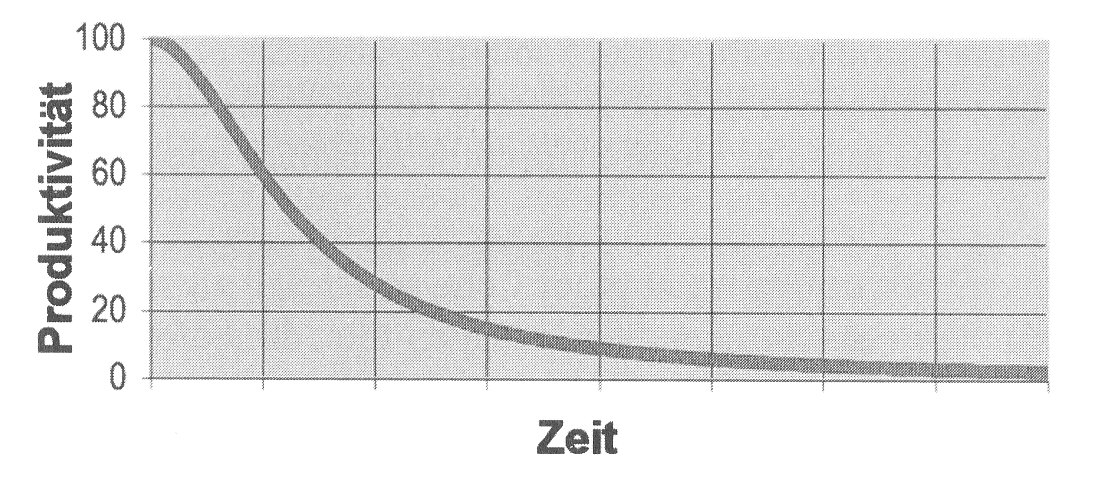
\includegraphics[width=\textwidth]{poduktivitaet.jpg}
	\caption{Produktivität über Zeit aus \cite[S. 29]{Martin}}
	\label{grundlagen:produktivitaet}
\end{figure}

Ein Entwickler der an einem solchen Quelltext arbeitet ist leicht versucht selbst schlechten Quelltext zu schreiben, da dies vermeintlich schneller geht und der Quelltext ohnehin schon nur schwer zu lesen ist. Daraus resultiert, dass der Quelltext immer unverständlicher wird und die Produktivität weiter sinkt.
Als möglicher Ausweg kommt eine Neuentwicklung der Software aus Sicht von \cite[S. 29f.]{Martin}, nicht in Frage.
Er begründet dies damit, dass neue Software neben der Weiterentwicklung der alten Erstellt werden muss und trotzdem auf denselben Funktionsumfang der alten Lösung kommen. Dies ist bei großen Softwareprojekten meistens nicht möglich, da bereit sehr viel Entwicklungszeit in das alte System geflossen ist und es zu teuer ist einen sehr großen Quelltext neu zu entwickeln. Als mögliche Lösung führt er an das jeder Entwickler versuchen sollten den Quelltext an den er gearbeitet hat sauberer als vorher zu hinterlassen. Er bezeichnet dies als Pfadfinderregel.

\subsection{Guter Quelltext}

Guten Quelltext zu schreiben ist etwas womit sich schon viele Entwickler beschäftigt haben\cite{Martin, Green, Spinellis, reed}.
\cite[S. 32f.]{Martin} hat sich mit den Aussagen von verschiedenen erfahrenen Entwicklern zu sauberem Quelltext auseinandergesetzt.
Er kommt zu folgenden Punkten für guten Quelltext:

\begin{itemize}
\item Testbar
\item Geradlinig, man erkennt den Zweck
\item Verständlich, einfach zu durchschauen, erwartungskonform
\item Keine versteckten Absichten
\item Gute Namen
\item Minimale Abhängigkeiten
\item Keine Redundanzen
\item Keine Fehler/Exceptions verstecken
\end{itemize}

Diese Punkte ähneln sehr stark den Design Ideen der Programmiersprache Python\cite{Peters}.
Wie anhand der Punkte zu erkennen ist, findet sich guter Quelltext auf verschiedenen Ebenen wieder. Auf unterster Ebene im Quelltext bis hin zur gesamten Architektur der Software. Häufig gehört allerdings ein hohes Maß an Erfahrung dazu einen guten Quelltext zu schreiben.


\subsection{Art and Science}

In vielen Artikeln zu dem Thema finden man die Wörter \enquote{Art} und \enquote{Science}. So z.B.
\enquote{Coding Guidlines: Finding the Art in Science} von \cite{Green} oder \enquote{Science and Art} von \cite[S. 669]{Knuth}.
Damit spielt man darauf an das manche Quelltexte sich so schön lesen und verstehen lassen, das es einer hohen Kunstfertigkeit bedarf sie zu schreiben. \cite[S. 669]{Knuth} zeigt, dass nicht nur die Informatik \enquote{Art} und \enquote{Science} in dieser weiße benutzt wird. Er fand es auch in einem Buch über die Grundlagen der Photographie und in der Einleitung eines Wörterbuches\cite[S. 669]{Knuth}.
Er zeigt zudem einen Wandel in der Verwendung des Wortes \enquote{Art}.
Früher war es üblich von einem gut ausgeführten Handwerk als Kunst zu reden.
Knuth zieht somit den Schluss, dass \enquote{Science} das Wissen ist und \enquote{Art} das angewandte wissen.
In unserem Fall ist das Programmieren das Handwerk und guter Quelltext die Kunst.
Weiterhin hat jeder Programmierer seinen eigenen Stil einen Quelltext zu schreiben.
Selbst Coding Conventions lassen dem Entwickler genug Freiraum für einen eigenen Schreibstil, da es nicht möglich ist alles mit ihnen zu definieren.


